\documentclass[journal]{IEEEtran}
\usepackage[a5paper, margin=10mm, onecolumn]{geometry}
\usepackage{lmodern}
\usepackage{tfrupee}
\setlength{\headheight}{1cm}
\setlength{\headsep}{0mm}

\usepackage{gvv-book}
\usepackage{gvv}
\usepackage{cite}
\usepackage{amsmath,amssymb,amsfonts,amsthm}
\usepackage{algorithmic}
\usepackage{graphicx}
\usepackage{textcomp}
\usepackage{xcolor}
\usepackage{txfonts}
\usepackage{listings}
\usepackage{enumitem}
\usepackage{mathtools}
\usepackage{gensymb}
\usepackage{comment}
\usepackage[breaklinks=true]{hyperref}
\usepackage{tkz-euclide}
\usepackage{listings}
\def\inputGnumericTable{}
\usepackage[latin1]{inputenc}
\usepackage{color}
\usepackage{array}
\usepackage{longtable}
\usepackage{calc}
\usepackage{multirow}
\usepackage{hhline}
\usepackage{ifthen}
\usepackage{lscape}
\usepackage{xparse}

\bibliographystyle{IEEEtran}

\title{8.2.7}
\author{EE25BTECH11043 - Nishid Khandagre}

\begin{document}
\maketitle

\renewcommand{\thefigure}{\theenumi}
\renewcommand{\thetable}{\theenumi}

\numberwithin{equation}{enumi}
\numberwithin{figure}{enumi}

\textbf{Question}:
Find the coordinates of the focus, vertex, eccentricity, axis of the conic section, the equation of the directrix and the length of the latus rectum. 
$16x^2 + y^2 = 16$

\textbf{Solution:}

We use an affine transformation to convert the conic equation to its standard form.
\begin{align}
    \vec{x}^\top\vec{V}\vec{x} + 2\vec{u}^\top\vec{x} + f = 0
\end{align}
The symmetric matrix $\vec{V}$ is spectrally decomposed to align axes with eigenvectors.
\begin{align}
    \vec{V} = \vec{P}\vec{D}\vec{P}^\top, \text{ } \vec{D} = \myvec{\lambda_1 & 0 \\ 0 & \lambda_2}, \text{ } \vec{P}^\top\vec{P} = \vec{I}
\end{align}
Substituting the decomposition into the conic equation.
\begin{align}
    \vec{x}^\top\vec{P}\vec{D}\vec{P}^\top\vec{x} + 2\vec{u}^\top\vec{x} + f = 0
\end{align}
A rotation
\begin{align}
    \vec{x_r} = \vec{P}^\top\vec{x} 
\end{align}
aligns the conic with the coordinate axes.
\begin{align}
    \vec{x} = \vec{P}\vec{x_r}
\end{align}
Applying the rotation to the conic equation.
\begin{align}
    \brak{\vec{P}\vec{x_r}}^\top\vec{P}\vec{D}\vec{P}^\top\brak{\vec{P}\vec{x_r}} + 2\vec{u}^\top\brak{\vec{P}\vec{x_r}} + f &= 0 \\
    \vec{x_r}^\top\vec{P}^\top\vec{P}\vec{D}\vec{P}^\top\vec{P}\vec{x_r} + 2\brak{\vec{P}^\top\vec{u}}^\top\vec{x_r} + f &= 0 \\
    \vec{x_r}^\top\vec{D}\vec{x_r} + 2\vec{u_r}^\top\vec{x_r} + f &= 0
\end{align}
A translation 
\begin{align}
    \vec{x_c} = \vec{x_r} + \vec{D}^{-1}\vec{u_r}
\end{align}
moves the conic's center to the origin.
\begin{align}
    f_c = f - \vec{u_r}^\top\vec{D}^{-1}\vec{u_r}
\end{align}
The center of the conic in the original coordinates is 
\begin{align}
    \vec{c} = -\vec{V}^{-1}\vec{u}
\end{align}
\begin{align}
    \vec{c} = -\brak{\vec{P}\vec{D}\vec{P}^\top}^{-1}\vec{u} = -\vec{P}\vec{D}^{-1}\vec{P}^\top\vec{u} = -\vec{P}\vec{D}^{-1}\vec{u_r}
\end{align}
The complete transformation from original to centered coordinates is 
\begin{align}
    \vec{x_c} = \vec{P}^\top\brak{\vec{x}-\vec{c}}
\end{align}
\begin{align}
    \vec{x_c} &= \vec{P}^\top\vec{x} + \vec{D}^{-1}\vec{u_r} = \vec{P}^\top\vec{x} - \vec{P}^\top\vec{c} = \vec{P}^\top\brak{\vec{x}-\vec{c}} \\
    \implies \vec{x} &= \vec{P}\vec{x_c} + \vec{c} \label{eq:71}
\end{align}
The given conic equation
\begin{align}
    16x^2 + y^2 = 16 \\
    \frac{16x^2}{16} + \frac{y^2}{16} = \frac{16}{16} \\
    \frac{x^2}{1} + \frac{y^2}{16} = 1
\end{align}
\begin{align}
    \vec{V} = \myvec{1 & 0 \\ 0 & \frac{1}{16}}, \text{ } \vec{u} = \myvec{0 \\ 0}, \text{ } f = -1
\end{align}
The major axis corresponds to smaller eigenvalue.
\begin{align}
    \lambda_1 = \frac{1}{16}, \text{ } \lambda_2 = 1, \text{ } \vec{P} = \myvec{0 & 1 \\ 1 & 0}, \text{ } \vec{c} = \myvec{0 \\ 0}
\end{align}
Applying the rotation to find the canonical coordinates.
\begin{align}
    \vec{x_c} = \vec{P}^\top\vec{x} \implies \myvec{x_c \\ y_c} = \myvec{0 & 1 \\ 1 & 0}\myvec{x \\ y} = \myvec{y \\ x}
\end{align}
The standard form of the ellipse in canonical coordinates.
\begin{align}
    \frac{x_c^2}{-f/\lambda_1} + \frac{y_c^2}{-f/\lambda_2} = 1
\end{align}
\begin{align}
    e &= \sqrt{1 - \frac{\lambda_1}{\lambda_2}} = \frac{\sqrt{15}}{4} \\
    \vec{f_c} &= \pm\sqrt{\frac{f\brak{\lambda_1 - \lambda_2}}{\lambda_1\lambda_2}}\vec{e_1} = \pm\sqrt{15}\vec{e_1} \\
    \vec{v_c} &= \pm\sqrt{\frac{-f}{\lambda_1}}\vec{e_1} = \pm 4\vec{e_1} \\
    \vec{d_c} &: \vec{e_1}^\top\vec{x_c} = \pm\sqrt{\frac{-f\lambda_2}{\lambda_1\brak{\lambda_2-\lambda_1}}} \pm\frac{16}{\sqrt{15}} \\
    L &= \frac{-2f}{\lambda_2}\sqrt{\frac{\lambda_1}{-f}} = \frac{1}{2}
\end{align}
Transforming properties back to the original coordinate system using \eqref{eq:71}
\begin{align}
    \vec{f} &= \vec{P}\brak{\pm \sqrt{15}\vec{e_1}} = \pm \sqrt{15}\vec{e_2} \\
    \vec{v} &= \vec{P}\brak{\pm 4\vec{e_1}} = \pm 4\vec{e_2} \\
    \vec{d} &: \vec{e_2}^\top\vec{x} = \pm \frac{16}{\sqrt{15}} \implies \myvec{0 & 1}\vec{x} = \pm \frac{16}{\sqrt{15}}
\end{align}
\begin{center}
\begin{tabular}{|l|c|}
    \hline
    \textbf{Property} & \textbf{Value} \\
    \hline
    Eccentricity & $\frac{\sqrt{15}}{4}$ \\
    \hline
    Axis & $x=0$ \\
    \hline
    Vertices & $\brak{0, \pm 4}$ \\
    \hline
    Foci & $\brak{0, \pm \sqrt{15}}$ \\
    \hline
    Directrices & $y = \pm \frac{16}{\sqrt{15}}$ \\
    \hline
    Latus Rectum & $\frac{1}{2}$ \\
    \hline
\end{tabular}
\end{center}






\begin{figure}[H]
	\centering
	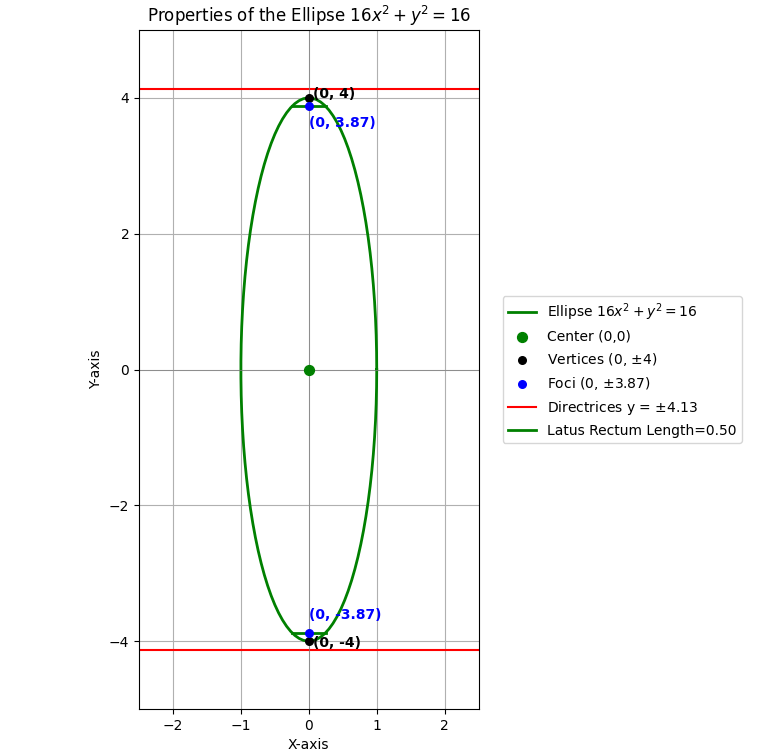
\includegraphics[width=0.8\columnwidth]{figs/fig1.png}
	\caption{}
	\label{fig:1}
\end{figure}

\end{document}
